\chapter{What the Commonwealth should do next}\label{chap:what_com_should_do}

This chapter details what the federal government should do in collaborative national efforts to ensure that education money is spent well. The Commonwealth’s biggest focus should be on delivering effectively in areas within its existing remit. Beyond that, the Commonwealth should do four specific things that would fill genuine gaps in Australia’s school education system. 

The proposed new national reforms should only be pursued if the states `buy in' and there is sustained Commonwealth-state collaboration in design and delivery.

\section{Deliver on existing federal responsibilities first}\label{sec:deliver-responsibilities}
The Commonwealth\space government can make significant contributions to school education through its existing areas of responsibility. It plays a large role in training teachers. The national curriculum, national student testing, high-quality data collection, and implementing professional standards in schools are all critical to the functioning of schools. All require constant attention, and some require urgent reform.

For example, the Commonwealth has much to do in improving initial teacher education, in line with recommendations of a major review in 2013.\footcite{2015AustralianGovernmentActionNowClassroomReadyTeachersReport}
A 2014 departmental review of the Australian Curriculum and Reporting Authority (ACARA) called for major changes to the National Report on Schooling.\footcite{2014AustralianGovernmentReviewoftheAustralianCurriculum}
And a 2016 Productivity Commission report on the National Evidence Base highlighted the important role the federal government plays in high-quality national data collection.\footcite{ProductivityCommission2016NationalEvidenceBase}
The Commonwealth\space government should act on recommendations such as these before embarking on new interventions into school education policy.

\section{Four specific national reforms}\label{sec:four-additional}

The following four reforms meet the three criteria set out in \Chapref{chap:few-reforms}. They do not `demand' specific inputs or outputs from the states. They are areas where increased scale and coordination is likely to result in big benefits for students. 
 
\subsection{Invest in measuring `new' capabilities}\label{subsec:new-capabilities}

Agreeing on the broad educational outcomes we want is seductively easy. But measuring progress in them is not. In many cases, Australia still lacks a concrete understanding of how to even teach non-cognitive skills, such as teamwork and resilience. As a result, we focus much more on measuring narrower foundational skills of literacy and numeracy, which are only an element of what we expect from schooling.

\begin{figure}
\caption{Giving teachers more `small data' will help}\label{fig:improve-how-to-measure}
\includegraphics[page=4]{charts/GonskiReportCharts.pdf}
\end{figure}

We must invest more in how to measure broader outcomes, and especially in `small data' for teachers to use in the classroom. The potential for big improvements is illustrated in \Vref{fig:improve-how-to-measure}. 

The Commonwealth should collaborate with states and territories on a major national research effort to improve how we measure these broader 21st century skills. Developing classroom measurement tools should be the first priority.  Every state and territory faces a similar challenge in this area, so it is appropriate for the Commonwealth\space government to invest and help coordinate this project in close collaboration with states and territories.

\subsection{Develop better measures of learning progress}\label{subsec:national-measure}

Australia needs better measures of student progress for national bench-marking and for use in the classroom.

NAPLAN seeks to measure students' learning progress in core literacy and numeracy skills at the national level, but NAPLAN gain scores are not easy to interpret when comparing the progress of different student groups. The Commonwealth\space government should develop a better measure of learning progress in NAPLAN for `big data' purposes.\footnote{Discussed in \textcite{Goss2016Wideninggapswhat}.}

The Commonwealth\space government should also develop a new `small data' progress measure for teachers to use in the classroom. This could be linked to the national curriculum and create consistency on what a year of learning progress looks like (new tools in this area are discussed in the next section).%
  \footcite{Goss2016Wideninggapswhat}
A 2011 OECD review of Australian policies highlighted the need for more `small data' to enhance student assessment in the classroom.%
  \footcite{OECD2011ReviewsofEvaluationandAssessmentinEducationAustralia}

\subsection{Invest in high-quality digital assessment tools for the classroom}\label{subsec:new-digital}

A consistent measure of progress in the classroom is one thing. But the tools to assess it are another. The Commonwealth\space government should invest in high-quality digital assessment tools that measure learning progress in the classroom. Quality assessment tools help to diagnose what students know, how much progress they have made, and how teaching can be improved to better meet students' needs. Measuring impact on student learning is the key to good decisions about what to keep and stop -- the selection process at the heart of an adaptive education system (see \Chapref{chap:Design_an_adaptive_system_of_continuous_improvement}).

Such tools should examine core academic skills (including a broad range of subject areas beyond literacy and numeracy), as well as new capabilities in critical thinking and non-cognitive skills. Given the curriculum is national, it is wasteful for each state (and many schools) to develop their own classroom assessment tools.\footcite{Goss2015TargetedTeachingHow} Any national efforts to develop new tools must be in consultation and close collaboration with state curriculum and assessment authorities, who should work in partnership with ACARA.

While the Commonwealth should improve teachers' access to assessment tools, the states and territories also need to ensure teachers have the capacity to interpret and use the assessment results to adjust their teaching -- a big issue in schools. Without complementary state government effort in this area, little is likely to change in teaching practice.

The Commonwealth\space government should also develop a `star' rating system for commercial assessment tools, to help schools choose the most appropriate new tools for their needs. Assessment experts should rate new products to help reduce individual school search costs (a large hidden cost).  This function could be done by existing bodies such as Education Services Australia or ACARA with appropriate extra funding for its delivery.

\subsection{Create a new national evidence body}\label{subsec:evidence-national} 

The Commonwealth should collaborate with the states to establish a new, national, independent research body that could encourage more evidence-based decision making in school education.

This body would complement, rather than replace, the existing network of state government research bodies. The Commonwealth would collaborate with states to establish the new organisation. Its functions would include sharing research findings across the country, setting national research priorities, lifting the standards for researchers, and helping to commission more rigorous research, trials and longitudinal surveys. Australia needs more and better education research; the Commonwealth should help fund it.\footnote{Of course any nationally commissioned research would have to be agreed to by state and territory governments and go through appropriate ethics approvals.} 

The new body could link-up all research on education for people from birth through to age 18, so there is a better understanding of the continuum of key learning stages from early childhood, school education through to  vocational education.

Specifically, the new national body should:

\begin{itemize}
    \item Coordinate research priorities and plan a long-term research agenda for school education
    \item Establish national evidence standards that encourage Randomised Controlled Trials (RCTs) and quasi-experiments
    \item Oversee high-quality research, trials and longitudinal surveys on ways to improve specific practices, in collaboration with state and territories (discussed in \Chapref{chap:Design_an_adaptive_system_of_continuous_improvement})
    \item Synthesise data and research findings so they are readily accessible to schools and policy makers
    \item Promote research findings through a range of media platforms and distribution channels.
    \item Bring researchers, schools and policy makers together so they can better understand the research and how to implement its lessons. \end{itemize}

The new body could be made up of a number of specialist branches; for example, one arm could specialise in evidence production and another in promotion (as done by the US Institute of Education Sciences).

It must be independent of government, for several reasons. Foremost, an independent body would be more likely to gain the trust of the education sector and the wider community. Teachers and school leaders are tired of government policies chopping and changing. They must be confident that the work of a national evidence body will not continually change with political tides. An independent body would help minimise political interference in the research agenda.

We do not agree with the Productivity Commission that ACARA is the best fit for a national evidence body, given the potential conflict of interest with its other functions.

Of course, independence does not necessarily guarantee quality. We agree with the criteria spelled out in the 2016 Productivity Commission report for selecting the appropriate governance arm.\footcite{ProductivityCommission2016NationalEvidenceBase}  

    

    
